\documentclass[11pt,twocolumn]{article}
\usepackage{caption}
\usepackage{anysize}
\usepackage{fancyhdr}
\usepackage{graphicx}
\usepackage{subcaption}
\usepackage{color}
\usepackage{balance}
\usepackage{lipsum}
\usepackage{multirow}
\usepackage{multicol}
\usepackage{booktabs}

\marginsize{.75in}{.75in}{.75in}{1in}
\pagestyle{fancy}
\rhead{\today}
\lhead{
\includegraphics[height=2.0cm]{logo.jpg}}
\rfoot{\thepage}
\cfoot{}
\renewcommand{\headrulewidth}{0pt} %removes line from fancy header
\renewcommand{\thispagestyle}[1]{} %placers header and footer on first page 
\renewcommand{\abstractname}{Summary}
\setlength{\columnsep}{25pt}
\date{}
\title{Laboratory Gasification Memo\\Biomass Moisture Experiments \vspace{-6ex}}

\begin{document}

\twocolumn[
  \begin{@twocolumnfalse}
    \maketitle
    \begin{abstract}
    
    Biomass gasification experiments using SEP Southern yellow pine of two different moisture levels were completed and analyzed.  The `low moisture' biomass has a moisture content of about 9-13\% by weight, and the `high moisture' biomass has a moisture content of about 18-23\% by weight.  It was discovered that higher moisture contents in the biomass led to better conversion across a wide range of space times at 1350 $^\circ$C.  

    \end{abstract}
  \end{@twocolumnfalse}
]

\section*{Experimental Methods}

In order to understand the effect of biomass moisture content on gasification, SEP Southern yellow pine with a high moisture content of around 18-23\% was tested at conditions mirroring tests done previously on dryer SEP Southern yellow pine with a moisture content of around 9-13\%.  Tests were completed over a wide range of space times and biomass flow rates of two, three, and four pounds per hour.

Pressure for all tests was 50 psig and temperature of the SiC outer wall was set at 1350 $^\circ$C.  Steam to biomass and CO$_2$ to biomass ratios were held constant as entrainment nitrogen flow rate was changed to adjust the space time.  Feedstock was sieved to a size of \textless 250 $\mu$m for both dry and wet experiments.  Detailed set points for all experiments can be found in Appendices \ref{app_dry_sp} and \ref{app_wet_sp}.

Four main results are discussed in this memo.  The first is total conversion, denoted as X$_{tot}$ in Equation \ref{eq_total}. This is a measure of the fraction of carbon in the biomass which is converted to any gaseous product. The carbon in the entrainment CO$_2$ is corrected for in the inlet and outlet so that unreacted CO$_2$ does not contribute to conversion totals.

\begin{equation}
	X_{tot} = \frac{\dot{n}_{C out,gas} - \dot{n}_{C_{in,CO_2}}}{\dot{n}_{C in,biomass}}
	\label{eq_total}
\end{equation}

Good conversion, X$_{good}$ in Equation \ref{eq_good}, is a measure of the fraction of carbon in the biomass which is converted to either CO or CO$_2$ .

\begin{equation}
	X_{tot} = \frac{\dot{n}_{C out,CO} + \dot{n}_{C out,CO_2}- \dot{n}_{C_{in,CO_2}}}{\dot{n}_{C in,biomass}}
	\label{eq_good}
\end{equation}

Methane yield is denoted as Y$_{CH_4}$ in Equation \ref{eq_ch4}. This equation calculates the fraction of carbon in the biomass which is converted to methane.

\begin{equation}
	Y_{CH_4} = \frac{\dot{n}_{C out,CH_4}}{\dot{n}_{C in,biomass}}
	\label{eq_ch4}
\end{equation}

Finally, tar load is given in Equation \ref{eq_tar}. It is a representation of the mass of benzene, toluene, and naphthalene measured in the outlet gas. $\dot{V}_{gas,out}$ is the volumetric flow rate of gas in standard cubic meters.

\begin{equation}
	Tar Load = \frac{\dot{m}_{C_6H_6} + \dot{m}_{C_7H_8}+ \dot{m}_{C_{10}H_8}}{\dot{V}_{gas,out}}
	\label{eq_tar}
\end{equation}

\section*{Results and Discussion}

\subsection*{Conversion}

Results for total and good conversions are shown in Figures \ref{plot_total} and \ref{plot_good}, respectively.  ANOVA on each of the results shows that both space time and moisture have a significant effect on the conversion calculations.  The ANOVA tests are outlined in Tables \ref{x_total} and \ref{x_good}.  It is clear that higher moisture content in the biomass leads to a higher conversion to CO and CO$_2$ in the experiments performed.

\begin{table}
	\centering
	\caption{Effects on total conversion for all tests.}
	\label{x_total}
	\begin{tabular}{c c}
	\toprule
	Effect				&	Prob \textless F	\\
	\midrule
	Space Time			&	\color{red}{\textless 0.0001} \\
	Moisture				&	\color{red}{\textless 0.0001} \\
	Space Time * Moisture	&	0.9067 \\
	\bottomrule
	\end{tabular}
\end{table}

\begin{figure}
\centering
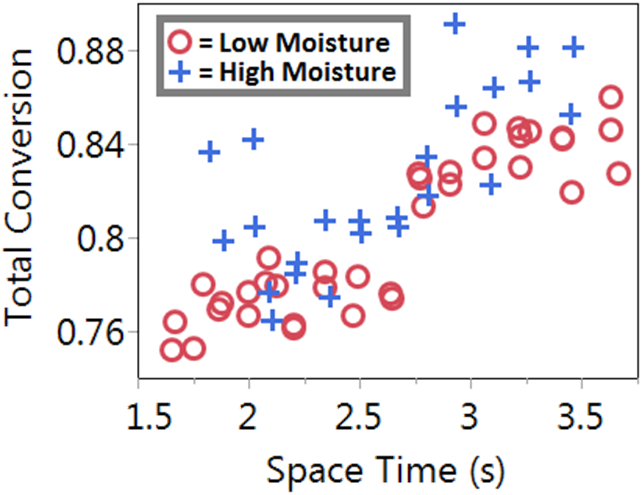
\includegraphics[width = 8cm]{x_tot.png}
\caption{Total conversion for biomass moisture experiments.}
\label{plot_total}
\end{figure}

\begin{table}
	\centering
	\caption{Effects on good conversion for all tests.}
	\label{x_good}
	\begin{tabular}{c c}
	\toprule
	Effect				&	Prob \textless F	\\
	\midrule
	Space Time			&	\color{red}{\textless 0.0001} \\
	Moisture				&	\color{red}{\textless 0.0001} \\
	Space Time * Moisture	&	0.1620 \\
	\bottomrule
	\end{tabular}
\end{table}

\begin{figure}
\centering
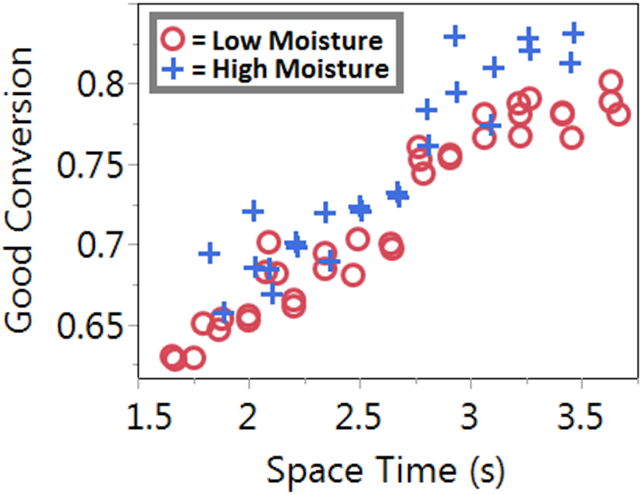
\includegraphics[width = 8cm]{x_good.png}
\caption{Good conversion calculations for biomass moisture experiments.}
\label{plot_good}
\end{figure}

\subsection*{Methane and Tars}

Analyzing all of the tests together using ANOVA shows that higher moisture content leads to lower methane yields (Table \ref{ch4}) but has no effect on tar loading (Table \ref{tar}).  However, looking at the plots for methane yield and tar loading shown in Figures \ref{plot_ch4} and \ref{plot_tar} suggests that the effects may be different depending on what space time regime one looks at.  Previous experience has also shown that methane yield tends to be correlated with tar yields.  If we see an effect on methane yield from biomass moisture, it might be expected that there is also an effect on tar yield.

\begin{table}
	\centering
	\caption{Effects on methane yield for all tests.}
	\label{ch4}
	\begin{tabular}{c c}
	\toprule
	Effect				&	Prob \textless F	\\
	\midrule
	Space Time			&	\color{red}{\textless 0.0001} \\
	Moisture				&	\color{red}{0.0014} \\
	Space Time * Moisture	&	\color{red}{0.0061} \\
	\midrule
	\end{tabular}
\end{table}

\begin{figure}
	\centering
	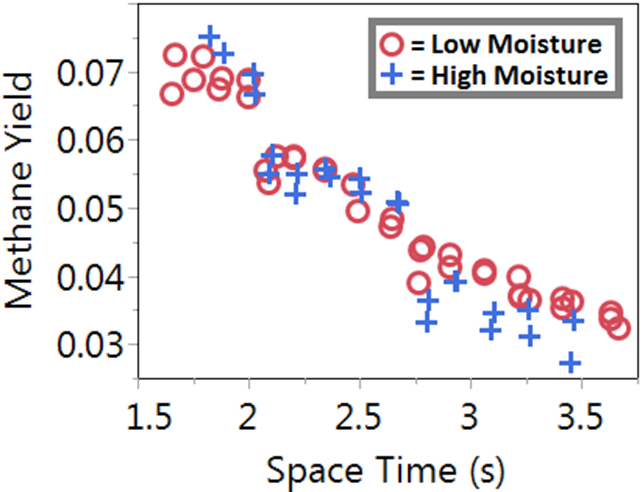
\includegraphics[width = 8cm]{ch4.png}
	\caption{Methane yield results for biomass moisture experiments.}
	\label{plot_ch4}
\end{figure}

\begin{table}
	\centering
	\caption{Effects on tar loading for all tests.}
	\label{tar}
	\begin{tabular}{c c}
	\toprule
	Effect				&	Prob \textless F	\\
	\midrule
	Space Time			&	\color{red}{\textless 0.0001} \\
	Moisture				&	0.1231 \\
	Space Time * Moisture	&	0.5562 \\
	\bottomrule
	\end{tabular}
\end{table}

\begin{figure}
	\centering
	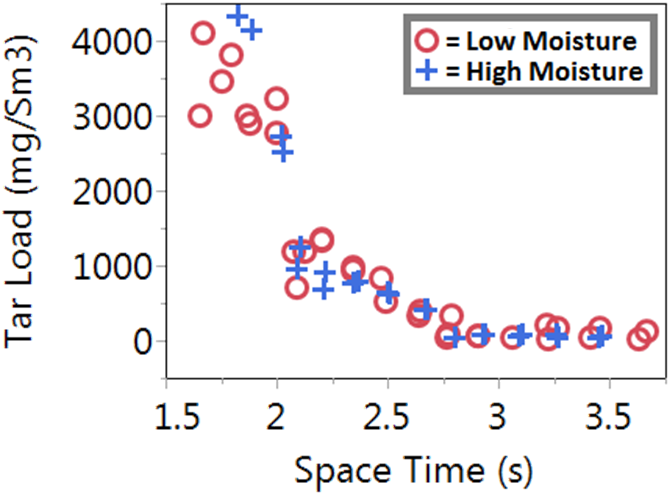
\includegraphics[width = 8cm]{tar.png}
	\caption{Tar loads for biomass moisture experiments.}
	\label{plot_tar}
\end{figure}

Performing ANOVA separately on 2, 3, and 4 lb/hr experiments shows interesting results for methane yield and tar loads.  At 2 lbs/hr, there is a negative effect on both methane and tar production from biomass moisture.  At 3 lbs/hr, an effect is not statistically detectable.  Then, at 4 lbs/hr, the effect from biomass moisture is positive in both methane and tar production.  These results are outlined in Table \ref{effect_summary}.  All tables giving detailed ANOVA results for each biomass flow rate are given in Appendix \ref{app_anova}.



\begin{table}
	\centering
	\caption{Summary of effect signs on methane yield and tar load for each biomass flow rate setpoint.}
	\label{effect_summary}

	\begin{tabular}{c c c c}
	\toprule
	& 2 lbs/hr &    3 lbs/hr &   4 lbs/hr   \\ 
	\midrule
	\multicolumn{1}{ c }{Methane}   & $-$ & {0} &  $+$ \\
	\multicolumn{1}{ c }{Tar}   & $-$ & {0} &  $+$ \\
	\bottomrule

	\end{tabular}

\end{table}

\subsection*{Moisture Effect on Carbon Content}

It's possible that there exists some sort of bias in the moisture measurements that could lead to errors in conversion calculations.  For example, if higher moisture biomass tended to read higher than the actual value while lower moisture biomass read at the actual moisture content, the calculated feed rate of carbon into the system would be lower than reality in higher moisture tests.  This could lead to higher conversion calculations.

To understand if the perceived difference in conversion for higher moisture biomass is due to analysis errors instead of physical effects, we can look at the dry carbon content for each biomass sample.  Each sample is tested for carbon content with included moisture content.  The dry carbon content is then reported by correcting for the moisture content which is found by the Karl-Fischer titration tests.  If there was a bias in the measured moisture content based on the moisture level, one would expect to be able to detect an effect of moisture level on dry carbon content.

ANOVA was run on the dry carbon contents to see if there was a difference in the means, and results are given in Table \ref{anova_moist}.  The average carbon content is 54.72\% on a dry basis for the low moisture tests and 55.13\% for high moisture biomass.  The probability that the means are different is well above an alpha value of 0.05, so it is safe to assume that moisture readings do not lead to a bias in conversion calculations.

\begin{table}
	\centering
	\caption{ANOVA results for dry carbon content for low and high moisture content biomass.}
	\label{anova_moist}
	\begin{tabular}{cccc}
	\toprule
	Moisture	& 	Mean \% C &  	Std Error	&	Prob \textgreater F \\
	\midrule
	Low		&	54.72	&	0.19		& 	\multirow{2}{*}{0.164}	\\
	High		&	55.13	&	0.22		& {} \\
	\bottomrule
	\end{tabular}
\end{table}

\subsection*{Discussion}

It was found that higher biomass moisture content has a positive effect on carbon conversion.  Chemically, this may be due to the proximity of surface bound water molecules to the biomass leading to faster reaction down more beneficial pathways.  It is also possible that there is a physical effect in which the bound moisture may be rapidly expanded to steam, causing biomass particles to expand or fracture.  This would raise the overall surface area of the biomass and lead to faster heat transfer rates.

At long space time regimes, there higher moisture content leads to lower tar and methane production.  An effect is not detected at mid-range space times and reverses so that higher moisture content leads to higher levels of methane and tars at very short space times.  It may be that,  at high flow rates, any benefits that surface moisture has on reducing tar and methane production may be outweighed by the vaporizing moisture leading to even shorter residence times.

While results may be due to an effect from the nature of the bound moisture in the biomass, they could also be due to the fact that there was simply more steam taking part in the reactions.  The inlet steam flow rates were not lowered to make up for the extra inlet water in the wet biomass.  Tests should be conducted in the future which take the extra water in the biomass into account and lower the steam flow rate to ensure all tests have similar total water flow rates.

Not accounting for the extra water in these experiments also means that the effective space times for the experiments are shorter than what is being calculated.  The addition of bound water which will quickly expand into steam will cause reactants to spend less time in the reactor.  Performing tests where the steam flow rate is lowered to account for the bound moisture will bring the space times more in line with lower moisture tests and may make the effects of bound moisture even more apparent.  

\section*{Conclusion}

Experiments have shown that increasing biomass moisture content and keeping all other set points equal leads to an increase in carbon conversion.  At long space times, methane production and tar yield are lowered as biomass moisture rises.  However, this effect flips so that higher moisture content leads to higher methane and tar levels at short space times.  It is recommended that tests be performed in the future which remove steam from the reactor inlet to take into account the extra water coming in with the biomass.  Keeping total water flow rates the same across wet and dry biomass tests can help to make clear if higher conversions are caused by higher partial pressures of steam or by the physical proximity of the bound moisture to the biomass.   

\balance

\newpage
\appendix
\onecolumn

\section{Experimental Set Points Dry Biomass}
\label{app_dry_sp}

\begin{center}
\begin{tabular}{ccccccccc}
\toprule
Run ID &  Temp 		&  Moisture 	&  Biomass 	&  Steam 	&  Steam 		&  Entrainment & Downbed	 & Argon \\
{}       & $^\circ$C	& \% wt		& lbs/hr		& ml/min	& $^\circ$C	& SLPM N$_2$	& SLPM CO$_2$	 & SLPM \\
\midrule
223    &       1350 &     12.85 &             2 &     12.08 &       300 &       27.18 &                3.3 &           2 \\
224    &       1350 &     12.85 &             2 &     12.08 &       300 &       15.10 &                3.3 &           2 \\
225    &       1350 &     12.85 &             2 &     12.08 &       300 &       12.08 &                3.3 &           2 \\
226    &       1350 &     11.86 &             2 &     12.08 &       300 &       18.12 &                3.3 &           2 \\
227    &       1350 &     11.86 &             2 &     12.08 &       300 &       12.08 &                3.3 &           2 \\
228    &       1350 &     11.86 &             2 &     12.08 &       300 &       15.10 &                3.3 &           2 \\
229    &       1350 &     11.86 &             2 &     12.08 &       300 &       18.12 &                3.3 &           2 \\
230    &       1350 &     11.86 &             2 &     12.08 &       300 &       21.14 &                3.3 &           2 \\
231    &       1350 &     11.86 &             2 &     12.08 &       300 &       24.16 &                3.3 &           2 \\
232    &       1350 &     11.86 &             2 &     12.08 &       300 &       21.14 &                3.3 &           2 \\
233    &       1350 &     11.86 &             2 &     12.08 &       300 &       27.18 &                3.3 &           2 \\
234    &       1350 &     10.67 &             2 &     12.08 &       300 &       24.16 &                3.3 &           2 \\
235    &       1350 &     10.67 &             4 &     24.16 &       300 &       24.16 &                6.6 &           2 \\
236    &       1350 &     10.67 &             4 &     24.16 &       300 &       18.12 &                6.6 &           2 \\
237    &       1350 &     10.67 &             4 &     24.16 &       300 &       36.24 &                6.6 &           2 \\
238    &       1350 &     10.60 &             4 &     24.16 &       300 &       36.24 &                6.6 &           2 \\
239    &       1350 &     10.60 &             4 &     24.16 &       300 &       24.16 &                6.6 &           2 \\
240    &       1350 &     10.60 &             4 &     24.16 &       300 &       30.20 &                6.6 &           2 \\
241    &       1350 &     10.60 &             4 &     24.16 &       300 &       18.12 &                6.6 &           2 \\
242    &       1350 &     10.70 &             4 &     24.16 &       300 &       30.20 &                6.6 &           2 \\
243    &       1350 &     10.70 &             3 &     18.12 &       300 &       31.71 &                4.9 &           2 \\
244    &       1350 &     10.50 &             3 &     18.12 &       300 &       27.18 &                4.9 &           2 \\
245    &       1350 &     10.50 &             3 &     18.12 &       300 &       27.18 &                4.9 &           2 \\
246    &       1350 &     10.50 &             3 &     18.12 &       300 &       18.12 &                4.9 &           2 \\
247    &       1350 &     10.50 &             3 &     18.12 &       300 &       22.65 &                4.9 &           2 \\
248    &       1350 &       9.29 &             3 &     18.12 &       300 &       18.12 &                4.9 &           2 \\
249    &       1350 &       9.29 &             3 &     18.12 &       300 &       13.59 &                4.9 &           2 \\
250    &       1350 &       9.29 &             3 &     18.12 &       300 &       13.59 &                4.9 &           2 \\
251    &       1350 &       9.29 &             3 &     18.12 &       300 &       31.71 &                4.9 &           2 \\
252    &       1350 &     11.07 &             3 &     18.12 &       300 &       22.65 &                4.9 &           2 \\
253    &       1350 &     10.50 &             3 &     18.12 &       300 &       31.71 &                4.9 &           2 \\
\bottomrule
\end{tabular}
\end{center}

\newpage
\section{Experimental Set Points Wet Biomass}
\label{app_wet_sp}

\begin{center}
\begin{tabular}{ccccccccc}
\toprule
Run ID &  Temp 		&  Moisture 	&  Biomass 	&  Steam 	&  Steam 		&  Entrainment & Downbed	 & Argon \\
{}       & $^\circ$C	& \% wt		& lbs/hr		& ml/min	& $^\circ$C	& SLPM N$_2$	& SLPM CO$_2$	 & SLPM \\
\midrule
363    &       1350 &     18.92 &             2 &     12.08 &       300 &       27.18 &                3.3 &           2 \\
364    &       1350 &     18.92 &             2 &     12.08 &       300 &       15.10 &                3.3 &           2 \\
366    &       1350 &     19.84 &             2 &     12.08 &       300 &       18.12 &                3.3 &           2 \\
368    &       1350 &     19.61 &             2 &     12.08 &       300 &       15.10 &                3.3 &           2 \\
369    &       1350 &     22.66 &             2 &     12.08 &       300 &       18.12 &                3.3 &           2 \\
370    &       1350 &     22.66 &             2 &     12.08 &       300 &       21.14 &                3.3 &           2 \\
371    &       1350 &     22.66 &             2 &     12.08 &       300 &       24.16 &                3.3 &           2 \\
372    &       1350 &     19.61 &             2 &     12.08 &       300 &       21.14 &                3.3 &           2 \\
373    &       1350 &     19.61 &             2 &     12.08 &       300 &       27.18 &                3.3 &           2 \\
374    &       1350 &     19.61 &             2 &     12.08 &       300 &       24.16 &                3.3 &           2 \\
404    &       1350 &     19.35 &             3 &     18.12 &       300 &       31.71 &                4.9 &           2 \\
405    &       1350 &     19.35 &             3 &     18.12 &       300 &       27.18 &                4.9 &           2 \\
406    &       1350 &     19.35 &             3 &     18.12 &       300 &       27.18 &                4.9 &           2 \\
407    &       1350 &     19.35 &             3 &     18.12 &       300 &       18.12 &                4.9 &           2 \\
408    &       1350 &     18.39 &             3 &     18.12 &       300 &       22.65 &                4.9 &           2 \\
409    &       1350 &     18.39 &             3 &     18.12 &       300 &       18.12 &                4.9 &           2 \\
410    &       1350 &     18.39 &             3 &     18.12 &       300 &       13.59 &                4.9 &           2 \\
411    &       1350 &     18.39 &             3 &     18.12 &       300 &       13.59 &                4.9 &           2 \\
412    &       1350 &     15.98 &             3 &     18.12 &       300 &       31.71 &                4.9 &           2 \\
413    &       1350 &     15.98 &             3 &     18.12 &       300 &       22.65 &                4.9 &           2 \\
414    &       1350 &     19.35 &             4 &     24.16 &       300 &       24.16 &                6.6 &           2 \\
415    &       1350 &     18.39 &             4 &     24.16 &       300 &       18.12 &                6.6 &           2 \\
418    &       1350 &     19.35 &             4 &     24.16 &       300 &       24.16 &                6.6 &           2 \\
420    &       1350 &     18.39 &             4 &     24.16 &       300 &       18.12 &                6.6 &           2 \\
421    &       1350 &     18.39 &             4 &     24.16 &       300 &       30.20 &                6.6 &           2 \\
\midrule
\end{tabular}
\end{center}

\section{Experimental Results}

\begin{center}
\begin{tabular}{ccccc}
\toprule
\multirow{2}{*}{Run ID} &  \multirow{2}{*}{Total Conversion} &  \multirow{2}{*}{Good Conversion} &  \multirow{2}{*}{Methane Yield} & Tar Loading \\
{}	&	{}	&	{}	&	{}	&	mg/Sm$^3$	\\
\midrule
223    &     0.8274 &      0.7602 &        0.03908 &            34.32 \\
224    &     0.8419 &      0.7817 &        0.03522 &            31.92 \\
225    &     0.8599 &      0.8011 &        0.03464 &            23.74 \\
226    &     0.8435 &      0.7812 &        0.03690 &            25.42 \\
227    &     0.8462 &      0.7887 &        0.03374 &            20.69 \\
228    &     0.8426 &      0.7810 &        0.03672 &            22.65 \\
229    &     0.8298 &      0.7675 &        0.03714 &            28.12 \\
230    &     0.8487 &      0.7812 &        0.04030 &            39.07 \\
231    &     0.8277 &      0.7558 &        0.04314 &            72.19 \\
232    &     0.8338 &      0.7666 &        0.04074 &            48.69 \\
233    &     0.8251 &      0.7528 &        0.04388 &            74.09 \\
234    &     0.8225 &      0.7542 &        0.04117 &            58.91 \\
235    &     0.7695 &      0.6467 &        0.06735 &             2991 \\
236    &     0.7766 &      0.6556 &        0.06888 &             3220 \\
237    &     0.7643 &      0.6278 &        0.07253 &             4095 \\
238    &     0.7523 &      0.6301 &        0.06678 &             2999 \\
239    &     0.7721 &      0.6535 &        0.06905 &             2902 \\
240    &     0.7527 &      0.6291 &        0.06882 &             3452 \\
241    &     0.7668 &      0.6530 &        0.06625 &             2768 \\
242    &     0.7799 &      0.6509 &        0.07229 &             3812 \\
243    &     0.7791 &      0.6817 &        0.05748 &             1183 \\
244    &     0.7612 &      0.6613 &        0.05764 &             1354 \\
245    &     0.7625 &      0.6650 &        0.05738 &             1325 \\
246    &     0.7668 &      0.6806 &        0.05341 &            841.9 \\
247    &     0.7853 &      0.6943 &        0.05572 &            986.2 \\
248    &     0.7833 &      0.7035 &        0.04945 &            516.2 \\
249    &     0.7741 &      0.6973 &        0.04839 &            403.1 \\
250    &     0.7759 &      0.7000 &        0.04719 &            337.6 \\
251    &     0.7914 &      0.7007 &        0.05358 &            710.0 \\
252    &     0.7784 &      0.6848 &        0.05555 &            940.4 \\
253    &     0.7809 &      0.6824 &        0.05550 &             1187 \\
\bottomrule
\end{tabular}

\begin{tabular}{ccccc}
\toprule
\multirow{2}{*}{Run ID} &  \multirow{2}{*}{Total Conversion} &  \multirow{2}{*}{Good Conversion} &  \multirow{2}{*}{Methane Yield} & Tar Loading \\
{}	&	{}	&	{}	&	{}	&	mg/Sm$^3$	\\
\midrule
363    &     0.8349 &      0.7836 &        0.03314 &            51.24 \\
364    &     0.8524 &      0.8126 &        0.02738 &            44.71 \\
366    &     0.8667 &      0.8203 &        0.03120 &            41.18 \\
368    &     0.8816 &      0.8319 &        0.03355 &            54.29 \\
369    &     0.8812 &      0.8282 &        0.03508 &            76.50 \\
370    &     0.8638 &      0.8105 &        0.03473 &            76.35 \\
371    &     0.8911 &      0.8299 &        0.03916 &            74.20 \\
372    &     0.8228 &      0.7744 &        0.03200 &            54.58 \\
373    &     0.8180 &      0.7618 &        0.03657 &            41.79 \\
374    &     0.8559 &      0.7950 &        0.03920 &            89.21 \\
399    &     0.8132 &      0.7439 &        0.04417 &            340.0 \\
400    &     0.8195 &      0.7666 &        0.03634 &            161.3 \\
401    &     0.8272 &      0.7806 &        0.03239 &            132.7 \\
402    &     0.8450 &      0.7906 &        0.03636 &            171.2 \\
403    &     0.8464 &      0.7878 &        0.03985 &            201.8 \\
404    &     0.7764 &      0.6843 &        0.05504 &            954.6 \\
405    &     0.7892 &      0.6987 &        0.05509 &            909.7 \\
406    &     0.7850 &      0.7009 &        0.05209 &            686.9 \\
407    &     0.8023 &      0.7203 &        0.05230 &            635.2 \\
408    &     0.8074 &      0.7197 &        0.05564 &            781.0 \\
409    &     0.8072 &      0.7240 &        0.05424 &            644.0 \\
410    &     0.8046 &      0.7290 &        0.05058 &            419.2 \\
411    &     0.8087 &      0.7324 &        0.05082 &            427.1 \\
412    &     0.7648 &      0.6691 &        0.05771 &             1244 \\
413    &     0.7746 &      0.6899 &        0.05459 &            785.2 \\
414    &     0.7986 &      0.6570 &        0.07270 &             4140 \\
415    &     0.8050 &      0.6861 &        0.06664 &             2514 \\
420    &     0.8419 &      0.7206 &        0.06958 &             2730 \\
421    &     0.8369 &      0.6948 &        0.07522 &             4338 \\
\bottomrule
\end{tabular}
\end{center}

\newpage
\section{ANOVA Results}
\label{app_anova}

\begin{table}[H]
	\centering
	\caption{Effects on methane yield for 2 lb/hr tests.}
	\label{tar2}
	\begin{tabular}{c c}
	Effect				&	Prob \textless F	\\
	\hline
	Space Time			&	\color{red}{\textless 0.0001} \\
	Moisture				&	\color{red}{0.0001} \\
	Space Time * Moisture	&	0.4605 \\
	\end{tabular}
\end{table}

\begin{table}
	\centering
	\caption{Effects on tar loading for 2 lb/hr tests.}
	\label{tar2}
	\begin{tabular}{c c}
	Effect				&	Prob \textless F	\\
	\hline
	Space Time			&	0.2853 \\
	Moisture				&	\color{red}{0.0280} \\
	Space Time * Moisture	&	0.6986 \\
	\end{tabular}
\end{table}

\begin{table}
	\centering
	\caption{Effects on methane yield for 3 lb/hr tests.}
	\label{tar2}
	\begin{tabular}{c c}
	Effect				&	Prob \textless F	\\
	\hline
	Space Time			&	\color{red}{\textless 0.0001} \\
	Moisture				&	0.6059 \\
	Space Time * Moisture	&	0.0918 \\
	\end{tabular}
\end{table}

\begin{table}
	\centering
	\caption{Effects on tar loading for 3 lb/hr tests.}
	\label{tar3}
	\begin{tabular}{c c}
	Effect				&	Prob \textless F	\\
	\hline
	Space Time			&	\color{red}{\textless0.0001} \\
	Moisture				&	0.2829 \\
	Space Time * Moisture	&	0.3581 \\
	\end{tabular}
\end{table}

\begin{table}
	\centering
	\caption{Effects on methane yield for 4 lb/hr tests.}
	\label{tar4}
	\begin{tabular}{c c}
	Effect				&	Prob \textless F	\\
	\hline
	Space Time			&	0.0638 \\
	Moisture				&	\color{red}{0.0277} \\
	Space Time * Moisture	&	0.7186 \\
	\end{tabular}
\end{table}

\begin{table}
	\centering
	\caption{Effects on tar loading for 4 lb/hr tests.}
	\label{tar4}
	\begin{tabular}{c c}
	Effect				&	Prob \textless F	\\
	\hline
	Space Time			&	\color{red}{0.0024} \\
	Moisture				&	\color{red}{ 0.0110} \\
	Space Time * Moisture	&	\color{red}{0.0170}  \\
	\end{tabular}
\end{table}


\end{document}

